\chapter{CASE STUDIES}
\label{chap:CaseStudies}

In this chapter, we explore the use of the DOI methodology in three concrete projects. We report on the instrumentation process, the data collection methods, and the research goals of these projects as a means of exemplifying the research processes that the DOI approach can facilitate.  

\section{Tracking Data Consumption in Visualization Systems}
\label{sec:ExperimentIMDB}
We study the degree to which the DOI approach can enable visualization researchers and analysts to track and understand what data users are foraging for, and what types of questions they are trying to answer while using interactive visualization systems. We showed that DOI data could reveal to an analyst, even in real-time, details about the tasks users are pursuing in an interactive visualization~\cite{Ala16, alam2015they}. We used this experiment to evaluate our first contributions (i.e. Section~\ref{sec:DOICollectionEvaluation}). 

To drive this research, we instrumented a Java-based PivotPaths~\cite{Dor12} visualization of movie data from the Internet Movie Database (IMDB). The visualization showed actors, movies, directors, and genres as 2D nodes connected by curves and was interactive. It could be zoomed and panned, users could select and highlight data, and could change the subset of data shown at any given time. 

We instrumented the visualization by inserting instructions that mirrored its modeling and rendering code so as to inform a viewed object detection module of the shapes, positions, and attributes (e.g., actor name, age, gender) of objects shown on the screen at any given time. We tracked individual data items (e.g., actor). The object detection module matched 2D gaze points received from an eye-tracker to screen objects reported by the visualization. We collected data from $9$ subjects using these visualizations interactively for thirty to forty-five minutes. The experimentation and instrumentation process is described in detail in Chapter~\ref{chap:DOIDataCollection}.

Typical questions we found that we were able to answer from DOI data were: ``Did a user try to solve a given task, or did they focus on specific data?'', ``Did a tracked user switch their analysis focus?'', ``When did a tracked user start solving a specific task?'', ``What data did users focus on when asked to solve a particular task?''. Such analyses can advance the visual analytics agenda by providing unprecedented insights into how users forage for and analyze data naturally, in interactive visual analytics systems and over extended periods of time. 

\section{Understanding Student Learning}
\label{sec:ExperimentArchitecture}
We work with education researchers to understand how students learn architecture using visual, interactive instruction material. In a preliminary pilot study with six subjects, we found that we can collect detailed DOI data from students learning via an interactive learning environment, to reveal the type of content learners focus on, and the sequences and patterns in which they do so. 

We explored an existing learning environment designed to teach architecture concepts related to facades and energy efficient building materials. This learning module was structured as an informational web application (HTML + Javascript), contained primarily text and images, and was interactive in that students could navigate between learning concepts, collapse and expand sections, and obtain details on demand. 

As described before, we instrumented the HTML and javascript code to allow the learning environment to permanently communicate (via AJAX protocols) to a viewed object detection module the shape, position, and nature (i.e., attributes) of the content it showed on the screen at any moment in time. As part of our experimental setup, students interacted with the web content on a local machine that we equipped with an eye-tracker. The detection module received gaze data from the eye-tracker and matched it to the visual content reported by the learning environment, to identify and record likely viewing targets.

Individual DOM elements with sufficient semantic meaning (e.g., paragraphs, images, headers, navigation widgets) formed the basis of DOI elements (Figure~\ref{fig:archictecture}). However, several images depicted complex schematics or included multiple panels. In such cases, we defined more granular DOIs within those pictures. 

We annotated DOIs with attributes such as which learning concept the DOI was referring to (e.g., facade, heat transmission, material type). Moreover, its complexity level (introductory, medium, advanced), the type of visual content it was depicted with (e.g., text, image, navigation widget), and the type of learning content (e.g., definition, example, exercise). The learning environment communicated These attributes to the instrumentation library, which in turn stored them as part of the description of viewed objects.

In our pilot experimental setup, six students spent approximately forty-five minutes exploring freely and absorbing the content illustrated in the learning module, as their gazes were tracked. In the end, their learning was quantified using a relatively short multiple choice questionnaire. Additionally, we collected information about students' educational background (e.g., pursued a major, career interests), degree progress (sophomore, junior, senior), and general demographic profile (e.g., age, gender).

This experimental setup and data collection process were designed to allow our collaborators to answer several high-level research questions expressed at our project's outset. These include: "Does a particular type or learning content or viewing pattern correlate with more efficient learning?"; "Does student background (e.g., engineering, science, arts) correlate with the type of content students focus on?"; "Are there viewing patterns that can predict learning deficiencies?". We hypothesize that the highly granular and annotated DOI data collected over extended periods of time from students learning "in the wild" from interactive visual content will facilitate insight different than that enabled by typical AOI-driven eye-tracking analyses.

\begin{figure}[htbp]
  \centering
  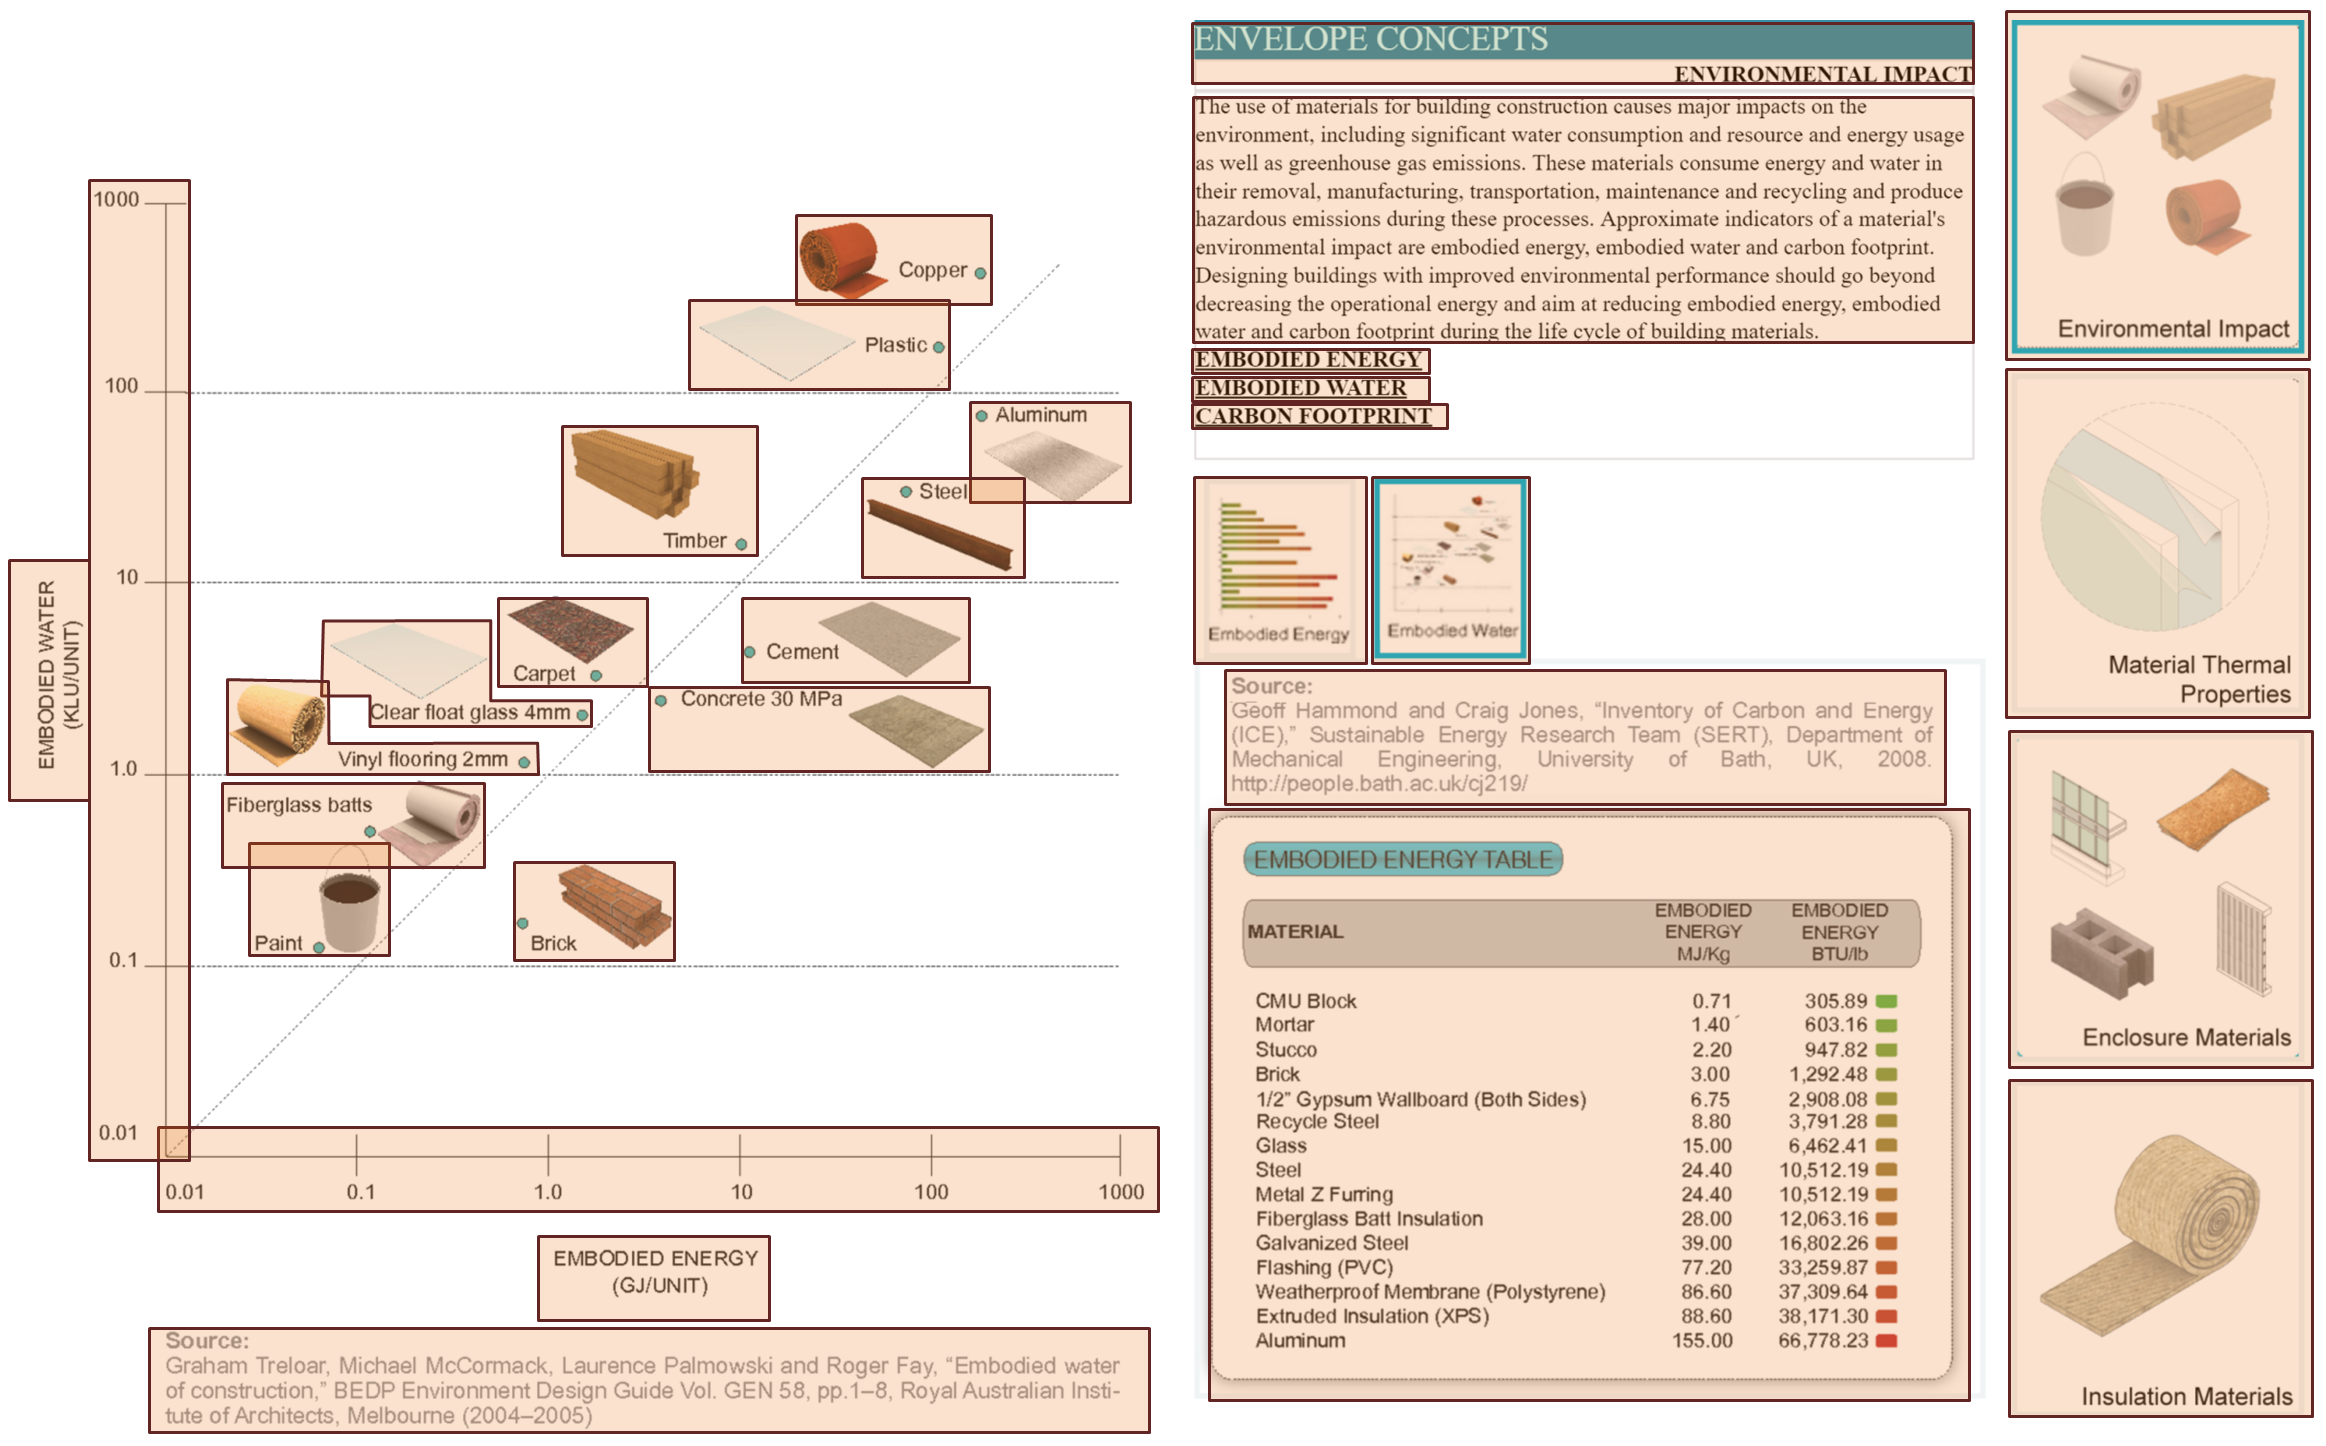
\includegraphics[width=\linewidth]{images/architectureDOI.eps}
  \caption{One page of an interactive, HTML environment for learning architecture concepts instrumented using our DOI instrumentation method from Chapter~\ref{chap:DOIDataCollection}. Overlays illustrate defined DOIs.}
	\label{fig:archictecture}
\end{figure}

\section{Exploring How Workers Detect and Assess Hazardous Situations on Construction Scenes}
\label{sec:ExperimentConstruction}
We collaborate with civil engineering researchers wishing to understand and model how construction workers identify and respond to safety hazards in construction scenes. Such research is important as the construction industry  suffers from the highest  number of  occupational fatalities  among all  the industries. 

Existing studies have explored the visual perception of workers on construction sites by tracking workers' gazes as they observe active sites for specific amounts of time~\cite{SafetyPerf}. However, simulating hazardous scenarios in-vivo is at best difficult, if not impossible. 
Moreover, capturing and analyzing eye-tracking data for videos is laborious, thus limiting previous experiments to short, constrained scenarios. 

Instead, we modeled a 3D construction scene from a real scene, using the Unity 3D framework, and had subjects explore this scene virtually on a computer screen, while an eye-tracker, in lieu with DOI instrumentation, captured which construction elements they observed. 

The scene was dynamic and involved multiple unfolding hazardous situations (e.g., a construction worker rushing in front of a vehicle). Subjects were assigned a virtual character which the scene placed in a truck that moved along a predetermined path through the scene (Figure ~\ref{fig:construction}). Subjects had no control over the transition of the camera (i.e., the truck's path), but they could change their viewing angle by rotating the camera in the horizontal plane. The whole 'trip' through the construction scene lasted approximately $8$ minutes. 

We instrumented the Unity scene using Bernhard et al.'s GTOM approach~\cite{Bern14}. Specifically, in addition to rendering the scene on the screen for subjects to view, we assigned each tracked object a specific color and rendered objects into a color buffer. We then identified colors in the proximity of gaze coordinates supplied by the eye-tracker and used this information to detect objects subjects potentially viewed. Figure~\ref{fig:construction} illustrates an example of the process.

Through the instrumentation process, we exported object attributes such as type (e.g., machinery, human, static), hazards associated with each object (e.g., collision, electrocution), whether objects were moving or not,  and their distance from the subject's camera. At the same time, we used the color buffers to compute the size of objects and their position (i.e., the center of mass) on the screen, and we tracked which of all objects were visible and which not. We note that the latter five types of attributes were time dependent. We also recorded screen captures and computed the bounds of objects on the screen. 

We collected such DOI data from sixteen subjects, half of which had construction training and the half which had not. Subjects were asked to complete a post-questionnaire about which hazardous situations they detected. Additionally, we collected subject-specific information such as experience and training levels. 

Specific questions that our collaborators expressed interest in, and that this experimental setup was designed to answer, included ``Viewing which types of visual items lead workers to identify specific hazards?'', ``How does the interest of experienced and novice construction workers in construction scene elements differ?'', ``Are there any low-level visual patterns that are unique to experienced construction workers?'', moreover, ``What types of hazards might go unnoticed at a construction site?''.

In addition to enabling the study of hazardous situations that are not safe to reproduce in vivo, we hypothesize that this DOI approach will eventually facilitate a novel, data-driven experimentation process. Specifically, our collaborators will be able to alter the construction scene often, between participant groups and in response to subjects' actions, or to simulate varied types of hazards and construction scene configurations, and document the resulting visual behavior. Examples of alterations include removing a virtual worker's reflective vest, altering the path of a worker to lead through a dangerous area, and removing or adding warning signs. Such experimentation can thus lend more significant data than traditional eye-tracking experimentation and facilitate novel workflows. While it is true that data collected in this way is of less ecological validity than that collected in situ, initial studies have shown that viewing patterns captured in virtual scenes may approximate those captured in real scenes well~\cite{nipesh}.

\begin{figure}[htbp]
  \centering
  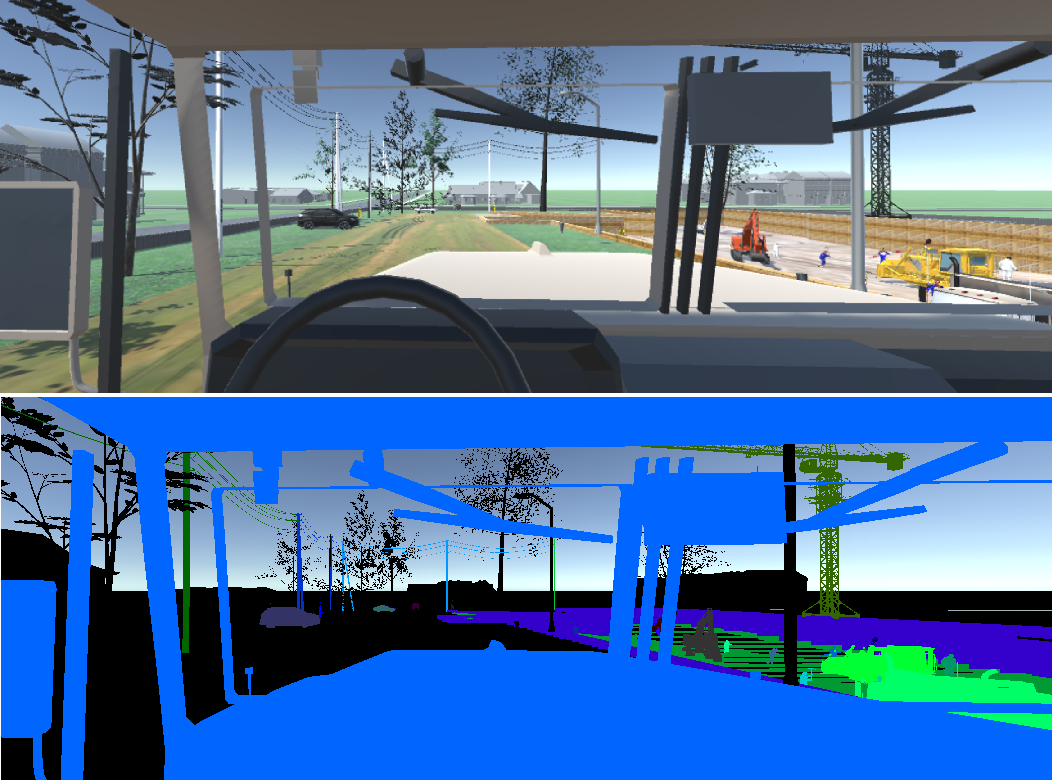
\includegraphics[width=\linewidth]{images/construction.eps}
  \caption{A 3D construction scene model (top) instrumented using Bernhard et al.'s color-buffer (bottom) approach~\cite{Bern14}. Each 3D object tracked in the scene is projected in the color buffer using a distinct color. Gazes are mapped to objects in the 3D space via their colors in the buffer.}
	\label{fig:construction}
\end{figure}

\section{Conclusions}
The analysis scope of eye-tracking data in any projects can be unbounded. Using real concepts have facilitated us on developing DOI analysis model and methods. All of the three projects mentioned in this chapter (Section~\ref{sec:ExperimentIMDB},~\ref{sec:ExperimentArchitecture}, and~\ref{sec:ExperimentConstruction}) have a general structure. Thus, many data analysis projects can relate to them. In this chapter, we discussed research workflow, analysis scope, visualization, and instrumentation methods. We will refer these projects as a basis for developing DOI data models and analysis framework in the following chapters. 